\documentclass[11pt]{article}
\usepackage{acl2016}
\usepackage{times}
\usepackage{latexsym}
\usepackage{amsmath, amssymb, amsthm, amsfonts}
\usepackage{multirow}
\usepackage[hidelinks]{hyperref}
\usepackage{hyperref}
\usepackage{float}
\usepackage{enumitem}
\setlist{nosep}
\usepackage{subcaption}
\usepackage{soul}
\hypersetup{
    bookmarks=false,         % show bookmarks bar?
    unicode=false,          % non-Latin characters in Acrobat’s bookmarks
    colorlinks=true,       % false: boxed links; true: colored links
    linkcolor=red,          % color of internal links (change box color with linkbordercolor)
    citecolor=black,        % color of links to bibliography
    filecolor=magenta,      % color of file links
    urlcolor=blue           % color of external links
}
\usepackage{tikz}
\usetikzlibrary{arrows,shapes,snakes,automata,backgrounds,petri,positioning}
\usepackage{pgfplots}

\aclfinalcopy

% To expand the titlebox for more authors, uncomment
% below and set accordingly.
% \addtolength\titlebox{.5in}    

\newcommand{\fix}{\marginpar{FIX}}
\newcommand{\new}{\marginpar{NEW}}
\newcommand{\NIL}{\mbox{\textsc{nil}}}
\newcommand{\qtext}[1]{\texttt{#1}}

\title{Collective Entity Resolution with Multi-Focal Attention}

\author{Amir Globerson\thanks{\;\;currently at Tel Aviv University} \and {\bf Soumen Chakrabarti}\thanks{\;\;currently at IIT Bombay} \and {\bf Nevena Lazic} \and \\ {\bf Amarnag Subramanya} \and {\bf Michael Ringgaard}
\and {\bf Fernando Pereira} \\ 
%Nevena Lazic \AND Amarnag Subramanya \and Michael Ringgaard \and Fernando Pereira \\
Google Inc., 1600 Amphitheatre Pkwy., Mountain View CA, 94043 \\
gamir@post.tau.ac.il, soumen@cse.iitb.ac.in, \\ $\{$nevena, asubram, ringgaard, pereira$\}$@google.com}

% Author information can be set in various styles:
% For several authors from the same institution:
% \author{Author 1 \and ... \and Author n \\
%         Address line \\ ... \\ Address line}
% if the names do not fit well on one line use
%         Author 1 \\ {\bf Author 2} \\ ... \\ {\bf Author n} \\
% For authors from different institutions:
% \author{Author 1 \\ Address line \\  ... \\ Address line
%         \And  ... \And
%         Author n \\ Address line \\ ... \\ Address line}
% To start a seperate ``row'' of authors use \AND, as in
% \author{Author 1 \\ Address line \\  ... \\ Address line
%         \AND
%         Author 2 \\ Address line \\ ... \\ Address line \And
%         Author 3 \\ Address line \\ ... \\ Address line}
% If the title and author information does not fit in the area allocated,
% place \setlength\titlebox{<new height>} right after
% at the top, where <new height> can be something larger than 2.25in


\date{}

\begin{document}
\maketitle

\begin{abstract}
Entity resolution is the task of linking each mention of an entity in
text to the corresponding record in a knowledge base (KB).  Coherence
models for entity resolution encourage all referring expressions in a
document to resolve to entities that are related in the KB. 
We explore attention-like mechanisms for coherence, where the evidence for each
candidate is based on a small set of strong relations, rather than relations
to all other entities in the document. 
The rationale is that document-wide support may simply not exist 
for non-salient entities, or entities not densely connected in the KB.
Our proposed system achieves 16--27\% relative reduction in error
compared to state-of-the-art systems on the CoNLL 2003, TAC KBP 2010, 2011
and 2012 tasks.
\end{abstract}

\newcommand{\be}{\begin{equation}}
\newcommand{\ee}{\end{equation}}
\newcommand{\bea}{\begin{eqnarray*}}
\newcommand{\eea}{\end{eqnarray*}}

\newcommand{\bean}{\begin{eqnarray}}
\newcommand{\eean}{\end{eqnarray}}


\renewcommand{\eqref}[1]{Eq.~(\ref{#1})}
\newcommand{\figref}[1]{Fig. \ref{#1}}
\newcommand{\secref}[1]{Sec. \ref{#1}}
\newcommand{\amax}{\text{amx}}
\newcommand{\samax}{\text{smx}}

\newtheorem{theorem}{Theorem}[section]
\newtheorem{lemma}[theorem]{Lemma}
\newtheorem{proposition}[theorem]{Proposition}

\newcommand{\reals}{\field{R}}
\newcommand{\field}[1]{\mathbb{#1}}
\newcommand{\phiv}{\boldsymbol{\phi}}

\newcommand{\fs}{\phiv_s(x,y_i)}
\newcommand{\fp}{\phiv_p(x,y_i,y_j)}
\newcommand{\ww}{\boldsymbol{w}} 
\newcommand{\vv}{\boldsymbol{v}} 
\newcommand{\ws}{\ww_s}
\renewcommand{\wp}{\ww_p}

\newcommand{\todo}[1]{({\textcolor{red}{#1}})}
\newcommand{\comment}[1]{}
\renewcommand{\exp}[1]{\text{exp}\left({#1}\right)}
\newcommand{\pdTwo}[2]{\frac{\partial#1}{\partial#2}}
\section{Introduction}
\label{sec:intro}

Entity resolution (ER) is the task of mapping mentions of entities in
text to corresponding records in a knowledge base (KB)
\cite{BunescuP06,Cucerzan07,KulkarniSRC09,Dredze2010,Hoffart2011,Hachey2013130}.
ER is a challenging problem because mentions are often ambiguous on
their own, and can only be resolved given appropriate context.  For
example, the mention \qtext{Beirut} may refer to the capital of
Lebanon, the band from New Mexico, or a drinking game
(Figure~\ref{fig:ereg}).
Names may also refer to entities that are not in the KB, a problem
 known as \emph{{\NIL} detection}.
% ER can improve text classification \cite{Gabrilovich2007}, information
% extraction \cite{Lin2012}, coreference resolution
% \cite{finin2009Coreference,mayfield2009cross} and other
% language-processing tasks.
%Kwiatkowski2011groundedsemparsing

Most ER systems consist of a \emph{mention model}, a \emph{context
  model}, and a \emph{coherence
  model}~\cite{Milne2008,Cucerzan07,Ratinov11,Hoffart2011,Hachey2013130}.
The mention model associates each entity with its possible textual
representations (also known as aliases or surface forms).  The context
model helps resolve an ambiguous mention using textual features
extracted from the surrounding context. 
%, such as the enclosing sentence and salient noun phrases in the document. 
The coherence model, which
is our focus in this work, encourages all mentions to resolve to
entities that are related to each other.  Relations may be established
via the KB, Web links, embeddings, or other resources.

Coherence models often define an objective function that includes
local and pairwise candidate scores, where the pairwise scores
correspond to some notion of coherence or relation
strength.\footnote{An exception to this framework are topic models in
  which a topic may generate both entities and words, e.g.,
  \cite{kataria2011,HanS12,houlsby2014scalable}.} 
  Support for a candidate is typically aggregated over
relations to all other entities in the document. One problem with this approach is that it may
dilute evidence for entities that are not salient in the document, or
not well-connected in the KB. This is an issue we aim to address.
%Finding an entity
% labeling that maximizes the objective is usually intractable and
% tackled via various approximations, which we discuss in more detail in
% Section~\ref{sec:related}. 



\begin{figure*}[!ht]
\centering
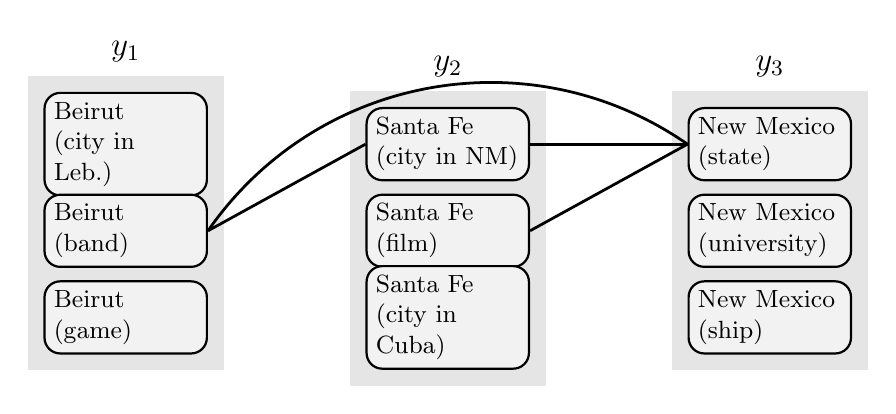
\begin{tikzpicture}[node distance=1.1cm and 2cm,>=stealth',auto]
  \tikzstyle{candidate}=[align=left,rectangle,rounded corners=2mm,thick,draw=black,fill=gray!10,minimum size=6mm,text width=52,font=\small]
  \tikzstyle{var}=[rectangle,thick,minimum size=6mm,font=\large]
  \tikzstyle{every label}=[black]

 \begin{scope}[-,line width=1pt]
    % First mention.
   \node [candidate] (c11){Beirut \\(city in Leb.)};
   \node [candidate] (c12) [below of=c11]  {Beirut \\(band)};
   \node [candidate] (c13)  [below of=c12] {Beirut \\(game)};
   \node [var] (y1) [above=0.2cm of c11] {$y_1$};

   % Second mention.
    \node [candidate] (c21) [right= of c11] {Santa Fe \\(city in NM)};
        \node [candidate] (c22) [below of=c21]  {Santa Fe \\ (film)};
    \node [candidate] (c23)  [below of=c22] {Santa Fe \\(city in Cuba)};
       \node [var] (y2) [above=0.2cm of c21] {$y_2$};
     
     % Third mention.
    \node [candidate] (c31) [right=of c21] {New Mexico \\(state)};
    \node [candidate] (c32)  [below of=c31] {New Mexico \\(university)};
    \node [candidate] (c33)  [below of=c32] {New Mexico\\ (ship)};
    \node [var] (y3) [above=0.2cm of c31] {$y_3$};
 
   \path (c12.east) edge (c21.west);
   \path (c12.east) edge [bend left=45] (c31.west);
   \path (c21.east) edge (c31.west);
   \path (c22.east) edge (c31.west);
   
  \end{scope}
  
  \begin{pgfonlayer}{background}
  \filldraw [fill=black!10,draw=black!10,line width=4mm]% [line width=4mm,black!10]
      (c11.north  -| c11.east)  rectangle (c13.south  -| c13.west)
      (c21.north -| c21.east) rectangle (c23.south -| c23.west)
      (c31.north  -| c31.east)  rectangle (c33.south  -| c33.west);
  \end{pgfonlayer}
\end{tikzpicture}
\caption{Illustration of the ER problem for three mentions ``Beirut'', ``New Mexico'' and ``Santa Fe''. each mention has three possible disambiguations. Edges link disambiguations that have Wikipedia links between their respective pages.}
\label{fig:ereg}
\end{figure*}



%The above coherence objectives consider the sum over all pairwise terms. Such
%``all-pairs'' coherence objectives aggregate over salient, well-connected
%entities and less prominent entities that are not so well-connected.
%In effect, all-pairs objectives seek evidence in favor of a candidate
%entity from \emph{all} other mentions in the document, evidence that
%may simply not exist for non-salient entities.  However, valuable
%support in favor of a candidate entity may be provided by a small
%number of entities chosen for other mentions.  Thus, all-pairs
%objectives risk losing these delicate signals.  Our primary goal is to
%fix this problem.

In this work, we introduce a novel coherence model with an attention mechanism, where the 
score for each candidate only depends on a small subset of mentions.
 Attention has recently been
used with considerable empirical success in tasks such as translation
\cite{bahdanau2014neural} and image caption generation
\cite{xu2015show}. We argue that attention is also desirable for
collective ER due to the discussed imbalance in the number of
relations for different entities.

Attention models typically have a single focus, implemented using the
 softmax function. Our model allows each candidate to
 focus on multiple mentions, and to implement it we introduce a 
 novel smooth version of the
 multi-focus attention function, which generalizes softmax.
%Our model relies on a novel smooth version of the multi-focus
%attention function, which generalizes the single-focus softmax
%function. 
%We use a simple and efficient inference procedure, and show
%how the model parameters can be learned from data.

We augment a competitive local context model (which does not use
coherence) similar to \cite{Lazic2015} with our coherence
framework, leading to performance improvements on three \todo{or four} evaluation benchmarks:
CoNLL 2003 \cite{Hoffart2011} and TAC KBP 2010--2012.
%On the CoNLL 2003 dataset \cite{Hoffart2011}, we see a relative
%reduction in error (RRIE) of \todo{FILL\%}.  On the TAC KBP 2010--2012
% datasets, we get a RRIE of in-KG entities around \todo{FILL\%}.

Our contributions thus consist of defining a novel multi-focal
attention model and applying it
successfully to an entity resolution system.  The approach can also be applied
to other structured prediction problems in language processing (such as
selecting antecedents in coreference resolution).  \todo{Move last sentence to conclusion?}

%Our premise is that this may also hold for entity relations:
%aggregating support for an entity label over the whole document may
%dilute the evidence for non-salient entities. We explore two new
%approaches to coherence that focus on a \emph{limited number} of
%relations for each candidate, rather than relations to all other
%entities.
%\begin{figure*}[!ht]
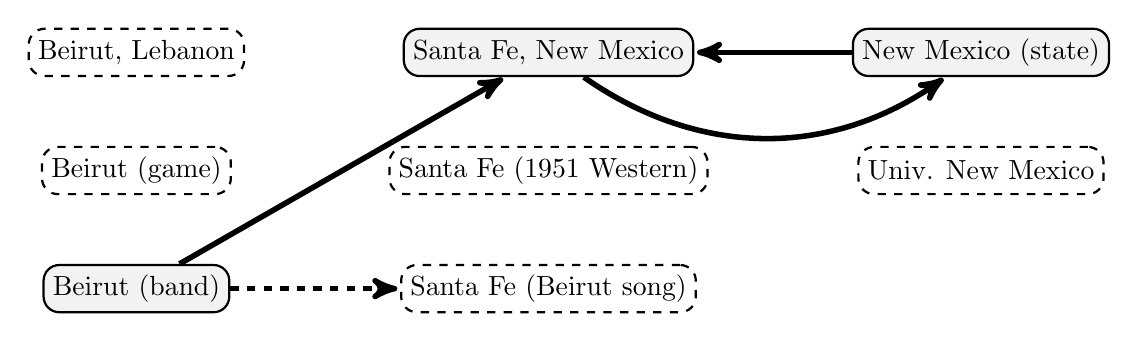
\begin{tikzpicture}[node distance=1.5cm,>=stealth',bend angle=35,auto]
  \tikzstyle{candidate}=[rectangle,dashed,rounded corners=2mm,thick,draw=black,fill=white,minimum size=6mm]
  \tikzstyle{selected} = [rectangle,rounded corners=2mm,thick,draw=black,fill=gray!10,minimum size=6mm]
  \tikzstyle{mention}=[rectangle,thick,draw=black!75,
  			  fill=black!10,minimum size=6mm]
  \tikzstyle{every label}=[black]

 \begin{scope}
    % First mention.
   % \node [mention] (m1){\qtext{Beirut}};
   % \node [candidate] (c11) [label=above:0.5] {Beirut, Lebanon};
   \node [candidate] (c11) {Beirut, Lebanon};
    \node [candidate] (c12) [below of=c11]  {Beirut (game)};
    \node [selected] (c13)  [below of=c12] {Beirut (band)};

   % Second mention.
   % \node [mention] [right=3cm of m1](m2){\qtext{Santa Fe}};
    \node [selected] (c21) [right=2cm of c11] {Santa Fe, New Mexico};
        \node [candidate] (c22) [below of=c21]  {Santa Fe (1951 Western)};
    \node [candidate] (c23)  [below of=c22] {Santa Fe (Beirut song)};

      
     % Third mention.
   % \node [mention] [right=3cm of m2](m3){\qtext{New Mexico}};
    \node [selected] (c31) [right=2cm of c21] {New Mexico (state)};
    \node [candidate] (c32)  [below of=c31] {Univ. New Mexico};
 
      
   %\path (c13) edge [post,line width=2pt] node[above]{0.5} (c21);
   \path (c13) edge [post,line width=2pt] (c21);
   \path (c13) edge [post,dashed,line width=2pt] (c23);
   \path (c31) edge [post,line width=2pt] (c21);
   \path (c21) edge [post,line width=2pt,bend right] (c31);
  \end{scope}
\end{tikzpicture}
\caption{Example coherency graph for mentions $\qtext{Beirut}$, $\qtext{Santa Fe}$ and $\qtext{New Mexico}$. Solid lines indicate a valid solution subgraph, where each selected candidate has at most one outgoing edge to another candidate. TODO: better example?}
\label{fig:graph}
\end{figure*}


%  Accordingly, we propose to choose the label for each mention based on the best support from a \emph{limited number} of other mentions.  In other words,  each mention is labeled by (tractable) inference in a star graph, but one where most edges are (dynamically) ignored.

\comment{
\subsection{Our contributions}
\label{sec:intro:our}

In the second \emph{attention} model, we allow each mention to have up to $K$ relations to other mentions. In this case, inference is tractable, and we also learn mention and edge scores from a small set of simple features.   %In other words,  each mention is labeled by (tractable) inference in a star graph, but one where most edges are (dynamically) ignored.

We use these coherence models to re-rank candidates generated by Plato \cite{Lazic2015}, a recent entity resolution system that has highly competitive performance and does not include a coherence component. This leads to performance improvements on three benchmarks, and yields new state-of-the-art results on the TAC KBP 2011 and 2012 datasets.
}


\secref{sec:notation} introduces notation.
\secref{sec:attention} presents the new multi-focus attention
model.  \secref{sec:maxsum} discusses a baseline model with
single focus.  \secref{sec:related} reviews related work.
\secref{sec:expt} presents experimental results.



%%% Local Variables: ***
%%% mode:latex ***
%%% TeX-master: "main.tex"  ***
%%% tex-main-file: "main.tex"  ***
%%% End: ***

\section{Definitions and notation}
\label{sec:notation}

We are given a document with $n$ mentions, where each mention $i$ has a set of $n_i$ candidate entities $\mathcal{C}_i = \{c_{i,1}, ..., c_{i,n_i}\}$. The goal is to assign a label $y_i \in \mathcal{C}_i$ to each mention.

Similarly to previous work, our approach to disambiguation relies on local and pairwise candidate scores. We denote the local score for mention $i$ by $s_i(y_i)$; this score is based only on local evidence, such as the mention phrase and surrounding textual features. The pairwise score for mentions $i$, $j$ is denoted by $s_{ij}(y_i, y_j)$,  and it is based on the relatedness of the two candidates. In Sections \ref{sec:score_param} and \ref{sec:learning} we discuss how these scores may be parameterized and learned.  Many systems that exploit coherence \cite{Cucerzan07,Milne2008,KulkarniSRC09} simply hardwire pairwise scores.

%In the \emph{single link} model, we compute these scores deterministically and use them as fixed model inputs. In the \emph{attention} model, we parameterize the scores and learn them using a labeled dataset.

Coherence models typically attempt to maximize a {\em global} objective function that assigns a score to each complete labeling ${\bf y} = (y_1,\ldots, y_n)$, given the local and pairwise scores. An example of such a function is the sum of all singleton and pairwise scores for the label:
 %A common example of such a function $g(y_1,\ldots,y_n)$ is:
\be
g({\bf y}) = \sum_i s_i(y_i) + \sum_i \sum_{j :  j \neq i} s_{ij}(y_i,y_j).
\label{eq:global_obj}
\ee 
One disadvantage of this approach is that maximizing $g$ corresponds to finding the maximum-a-posteriori (MAP) assignment of a general pairwise Markov random field, and is hence
NP hard for the general case \cite{wainwright2008graphical}. Another limitation is that non-salient entities may only have a few relations in a document, and summing over all mentions may dilute the evidence for such entities. In this paper we explore alternative optimization objectives, relying on attention and tractable inference.



%%% Local Variables: ***
%%% mode:latex ***
%%% TeX-master: "main.tex"  ***
%%% tex-main-file: "main.tex"  ***
%%% End: ***



\section{Attention model}

Assume we have $n$ mentions we wish to disambiguate. The $i^{th}$ mention will have $n_i$ candidates and we denote those by $c_1,\ldots, c_{n_i}$. The goal 
of the entity linking model is to assign a label $y_i\in \{c_1,\ldots, c_{n_i}\}$ to each mention.

As with other coherence based approaches, we use local and pairwise scores. Local scores are denoted by $s_i(y_i)$, and score each candidate $y_i$ for the $i^{th}$ mention based on local evidence (e.g., context, mention text etc). The pairwise scores are denoted by $s_{i,j}(y_i,y_j)$ and score each candidate pair based on its coherence. 

In what follows, we first describe the inference part of our model. Namely, how to predict the labels $y_i$ given the scores. We later explain how scores are calculated and learned.

\subsection{Inference}
One approach to coherence modeling is to maximize a {\em global} objective function, that assigns a score to each complete labeling $y_1,\ldots,y_n$.
 A common example of such a function $g(y_1,\ldots,y_n)$ is:
\be
\sum_i s_i(y_i) + \sum_{i\neq j} s_{ij}(y_i,y_j)
\label{eq:global_obj}
\ee 
One disadvantage of this approach is that it maximizing $g$ takes type exponential in $n$. Another, as we discuss later, is that it sums information across all entities and can introduce noise in the process, which our attention model can overcome.

\subsubsection{The Star Model}
To avoid the computational hardness, we first consider a simpler inference procedure, which we call a {\em star model}. We will later introduce attention into the model, but begin with the attention free case. Our approach labels each $y_i$ separately. To label $y_i$ we consider a star shaped graphical model, which is centered at $y_i$, as illustrated in \figref{fig:star}. The corresponding score function is:
\be
f_i(y_1,\ldots,y_n) = \sum_j s_j(y_j) + \sum_{j\neq i} s_{ij}(y_i,y_j) ~,
\label{eq:star_obj}
\ee
and the label $y_i$ is obtained by maximizing over all labels, and returning that of $y_i$. Namely:
\be
y_i = \arg\max_{y_i} \max_{y_{j}: j\neq i} f_i(y_1,\ldots,y_n)
\ee
Since $f_i$ corresponds to a star shaped graphical model, maximization is easy and can be done in $O(nC^2)$, where $C$ is the maximum number of candidates.

\subsubsection{Adding Attention \label{sec:add_attention}}
The score function in \eqref{eq:star_obj} aggregates scores from all other mentions $j\neq i$, in order to label mention $i$. If the document has many mentions, this can introduce noise into the decision process. To reduce this effect, we introduce attention into our model, and allow it to only use scores from mentions that have high coherence with $y_i$. We next define this notion more formally. 

We specify a parameter $K$, that denotes the maximum number of mentions to attend to. Next, define the function $\amax(z_1,\ldots,z_n)$ to be
the sum of the top $K$ values in $z_1,\ldots,z_n$.  For each $j\neq i$, we define the coherency between $y_i$ and $j$ to be:
\be
s_{ij}(y_i) = \max_{y_j}  s_{ij}(y_i,y_j)  + s_j(y_j)
\ee
Where we also define $s_{ii}(y_i)=-\infty$ to simplify notation later. Thus, $s_{ij}(y_i)$ gives the strength of support that mention $j$ gives to candidate $y_i$. Since we want to only attend to the most informative mentions, we will only consider  the $K$ best mentions. Namely, we consider the score function:
\be
f_i(y_i) = s_i(y_i) + \amax(s_{i1}(y_i), \ldots, s_{in}(y_i))
\label{eq:amax_obj}
\ee
Labeling is then simply done by taking the argmax of $f_i(y_i)$. Computationally, the cost is $O(nC^2+ n\log{n})$ since sorting is required.\footnote{Note that if $k < \log{n}$, we can use $nk$ instead of $n\log{n}$.}  

\subsubsection{Soft Attention \label{sec:soft_attention}}
Several works on attention have shown that it is better to use a soft form of attention, where the level of attention is not zero or one, but can rather take intermediate values. In current attention models, the attention is to a single object (e.g., a word as in \cite{} or part of an image as in \cite{}). In these cases, it is natural to change the max function in the attention operator to a soft-max. In our case, the attention beam contains $K$ elements, and we require a different notion of a soft-max, which we develop below.

Our goal is to obtain a soft-version of the function  $\amax(z_1,\ldots,z_n)$. To do so, we first use an alternative definition of this function, as the solution 
to the optimization problem:
\be
 \max_{ 
\begin{array}{l}
x_1,\ldots,x_n: \\
0 \leq x_i \leq 1\\
 \sum_i x_i = K
 \end{array}
 } \sum_i z_i x_i
\ee
The optimization problem above is a linear program, whose solution is the top $K$ element of $z$ as required. This follows, since $x_i$ at the optimum can easily be seen to attain only integral values (otherwise the objective can be improved. Alternatively, it can be shown that the vertices of the constraining polytope are integral).

Given this optimization view of $\amax(z_1,\ldots,z_n)$ it is natural to smooth it \cite{Nesterov} by adding a non-linearity to the optimization. A very natural choice
is an entropy regularizer, which also recovers the standard soft-max case for $K=1$.  Consider the optimization problem:
\be
 \max_{ 
\begin{array}{l}
x_1,\ldots,x_n: \\
0 \leq x_i \leq 1\\
 \sum_i x_i = K
 \end{array}
 } \sum_i z_i x_i + \beta \sum_i x_i \log{x_i}
\ee
We denote its solution by $\samax(z_1,\ldots,z_n)$. The following proposition provides a closed form solution for $\samax$, as well as its gradient.

\begin{proposition}
Assume $i_1,\ldots,i_n$ are such that $z_{i_1}\geq \ldots \geq z_{i_n}$. Then:
\be
\samax(z_1,\ldots,z_n) = \sum_{j=1}^{K-1} z_{i_j} + \beta \log\sum_{j=K} e^{\beta^{-1} z_{i_j}}  
\ee
Furthermore, $\samax(z_1,\ldots,z_n)$ is differentiable and its gradient is given by $....$ 
\end{proposition}  
Proof is provided in the appendix.

Note that when $K=1$, we recover the standard soft-max function \cite{}. For other $K$, the function $\samax$ has an intuitive interpretation: take the sum of the top $K-1$ elements of $z_1,\ldots,z_n$, and add the soft-max of all other elements. As $\beta\to 0$, this soft-max will approach the true max and therefore the soft-max of the suffix will be exactly the $K^{th}$ top element, and $\samax$ will therefore be the sum of the top $K$ elements as expected. For finite $\beta$ we have a soft version of $\amax$.

Our soft attention based model will therefore consider the soft-variant of \eqref{eq:amax_obj} 
\be
f_i(y_i) = s_i(y_i) + \samax(s_{i1}(y_i), \ldots, s_{in}(y_i)) ~,
\label{eq:samax_obj}
\ee
and maximize $f(y_i)$ to obtain the label.
 
\subsection{Score Parameterization}
Thus far we assumed the singelton and pairwise scores were given. As in other structured prediction works, we will assume that the scores are features of the input and labels. Specifically, denote a set of singleton features by $\fs\in\reals^{n_s}$ and a set of pairwise features by $\fp\in\reals^{n_p}$. Then the model has two sets of weights $\ws$ and $\wp$ and the scores are obtained as a linear combination of the features. Namely:
\bea
s_i(y_i;\ws) &=& \ws\cdot\fs  \\
s_{ij}(y_i,y_j;\wp) &=& \wp\cdot\fp ~, \\
\eea
where we have expicitly denoted the dependence of the scores on the weight vectors. See \secref{sec:features} for details on how the features are chosen. It of course possibel to consider non-linear alternatives for the score function, as in recept works \cite{manning,neurosis}, but we focus on the linear case for simplicity.

\subsection{Parameter Learning}
The parameters $\ws,\wp$ are learned from labeled data, as explained next. Since prediction is performed for each mention separately, we use a simple hinge loss for that mention. The loss is defined as follows. Denote by $y^*_i$ the ground
truth label for mention $i$. Define the corresponding ground truth $s_{ij}$ as:
\be
s^*_{ij} = s_{ij}(y^*_i,y^*_j)
\ee
Then the hinge loss is:
\bea
\ell_i &=& \max_{y_i}[ s_i(y_i) + \samax(s_{i1}(y_i), \ldots, s_{in}(y_i))  \\
       && - s_i(y^*_i) - \samax(s^*_{i1}, \ldots, s^*_{in})  
       + \Delta(y_i,y^*_i) ]
\eea
where $\Delta(y_i,y^*_i)$ is zero if $y_i=y^*_i$ and one otherwise.

The overall loss is simply the sum of loss for all the mentions, plus $\ell_2$ regularization over $\ws,\wp$. To minimize the loss we use AdaGrad \cite{adagrad} with learning rate $\eta=0.1$.


\section{Single-link model}
\label{sec:maxsum}

To motivate our modeling choices of using multi-focal attention and decomposed inference, we additionally consider a simple baseline model with single-focus attention and global inference. In this approach, which we name \emph{single link}, each mention $i$ attends to exactly one other mention that maximizes the pairwise relation score. The corresponding objective can be written as
\begin{align}
g^{SL}({\bf y}) &= \sum_i \bigg( s_i(y_i) + \max_{ j | j \neq i} s_{ij}(y_i, y_j) \bigg).
\end{align}

While exact inference in this model remains intractable, we can find approximate solutions using max-sum belief propagation \cite{Kschischang2001}. 
As a reminder, max-sum is an iterative algorithm for MAP inference which can be described in terms of messages sent from model factors $g_a({\bf y}_a)$ to each of their variables $y \in {\bf y}_a$. At convergence, each variable is assigned to the value that maximizes \emph{belief} $b(y)$, defined as the sum of incoming messages. The message updates have the following form:
\begin{align}
\mu_{g_a \rightarrow Y}(y) =& \max_{ {\bf y}_a \setminus y } \bigg[ g_a({\bf y}_a) + \sum_{j \neq i} q_j^{\setminus a}(y_j)\bigg]
\label{eq:damping}
\end{align}
\noindent where $q_j^{\setminus a}(y_j)$ is the sum of all messages to $y_j$ except the one from factor $g_a$. 
While the single-link model contains global factors $\max_{ j | j \neq i} s_{ij}(y_i, y_j)$ over $n$ variables, computing the messages from these factors is tractable and requires sorting.


%%% Local Variables: ***
%%% mode:latex ***
%%% TeX-master: "main.tex"  ***
%%% tex-main-file: "main.tex"  ***
%%% End: ***

\section{Related work}
\label{sec:related}

\subsection{Coherence scores}

Several systems \cite{Milne2008,KulkarniSRC09,Hoffart2011} use the ``Milne and Witten'' measure for relatedness between a pair of entities, which is based on the number of Wikipedia articles containing each entity, and the number of articles containing both; \cite{Cucerzan07} has also relied on the Wikipedia category structure. %The overall coherence score of a candidate is then computed as a weighted average of such similarities. 
Wikipedia also provides direct evidence of relatedness between a pair of of entities by way of intra-Wikipedia links from the page of one entity to another. Another source of information are Web pages containing links to Wikipedia pages of both entities (although the signal here may be more noisy); such links have been used in several recent systems \cite{ChengR13,Chisholm2015}.  Yet another attractive alternative, in few of the recent success of deep learning, is to build continuous vector representations of entities, and use those to define a pairwise similarity between entities \cite{YamadaS0T16}.


\subsection{Collective inference for ER}

As discussed earlier, optimizing most reasonable coherence objectives is intractable. \newcite{Milne2008} and \newcite{Ferragina10} decompose the problem over mentions and select the candidate that maximizes their relatedness score, but that involves extending attention to \emph{all} other mentions ($K=n-1$).  \newcite{Hoffart2011} extract a dense subgraph from the original graph by using an iterative heuristic to remove unpromising mention-entity edges. \cite{Cucerzan07} creates a relation vector for each candidate, and disambiguates each entity to the candidate whose vector was most similar to the aggregate (which includes both correct and incorrect labels). \newcite{KulkarniSRC09} formulate the task as an integer linear program and find solutions via a convex relaxation, while \newcite{ChengR13} directly use an integer linear program solver. A shortcoming of these approaches is that they may be too slow \hl{check} for Web-scale ER. \newcite{Ratinov11} use relation scores as features in a ranking support vector machine.
 
Personalized PageRank (PPR) \cite{jeh2003scaling} is another tractable alternative to collective inference, adopted by several recent systems \cite{Han2011,He13,Alhelbawy14,Pershina2015}. A closely related approach is Laplacian smoothing \cite{Huang2014}.  In most applications of PPR to ER, the graph and edge weights are fixed a-priori, and there is no dynamic association between $y_i$ and the best supporting mentions~$j$.

%Common shortcomings of these systems include the absence of a convincing generative or discriminative story that integrates local and coherence signals.  Typically, there is no training for the PPR part of the score; it is hardwired into the final labeling process. 

\subsection{Attention models}
Attention based models have recently shown great promise in several applications, such as machine translation \cite{bahdanau2014neural} and image caption generation \cite{xu2015show}.  In both these domains, attention is used to choose which information is relevant for producing the next work. Our work introduces a significantly different attention mechanism, which considers multiple foci of attention, and generalizes previous soft attention approach to handle those. Furthermore, we optimize
over the attention foci and the predicted label jointly, and not in a feed-forward manner as done in previous works.

Here we consider attending to different mentions in a document. We note that systems such as \newcite{Jin:2014} and \newcite{Lazic2015} may be viewed as
attending to single context features, via a model that is very different from ours, and not readily extendible to attention to mentions.

%which perform per-instance feature selection and argue that many context features of a mention can be unnecessary or even detrimental. 

%\paragraph*{Heuristics:}
%\cite{Cucerzan07} avoided the combinatorial explosion by aggregating profile vectors representing all candidates for all mentions other than the one being labeled, and then choosing the entity label whose profile vector was most similar to the aggregate.   But the aggregates were therefore superpositions of profiles of correct and incorrect labels.  \cite{KulkarniSRC09} used hill-climbing.  \cite{Hoffart2011} also used an iterative heuristic to remove unpromising mention-entity edges and thus extract a dense subgraph from the original graph.

%\paragraph*{Optimization/learning:}
%\newcite{KulkarniSRC09} formulated the task as an integer linear program and found solutions via a convex relaxation, while \newcite{ChengR13} directly used an integer linear program solver.  These approaches worked in practical amounts of time, but were too slow \hl{check} for Web-scale NERD \cite{Lazic2015}.  \newcite{Ratinov11} use relation scores as features in a ranking support vector machine.

%\paragraph*{Personalized PageRank (PPR):}
%Personalized PageRank (PPR) \cite{jeh2003scaling} is another tractable alternative to (combinatorial) collective inference, adopted by several recent systems \cite{Han2011,He13,Alhelbawy14,Pershina2015}. A closely related approach is Laplacian smoothing \cite{Huang2014}.  Common shortcomings of these systems include the absence of a convincing generative or discriminative story that integrates local and coherence signals.  Typically, there is no training for the PPR part of the score; it is hardwired into the final labeling process. 



%Our approach to coherence is partly inspired by the systems reported by \cite{Jin:2014} and \cite{Lazic2015}, which perform per-instance feature selection and argue that many context features of a mention can be unnecessary or even detrimental.


%%% Local Variables: ***
%%% mode:latex ***
%%% TeX-master: "main.tex"  ***
%%% tex-main-file: "main.tex"  ***
%%% End: ***

\section{Experiments}
\label{sec:expt}

\subsection{Evaluation data}

\paragraph*{CoNLL:} 
The CoNLL dataset ~\cite{Hoffart2011} contains 1393 articles with
about 34K mentions, and the standard performance metric is
mention-averaged accuracy.  The documents are partitioned into train,
test-a and test-b. Like most authors, we report performance on the
231 test-b documents with 4483 linkable mentions.  


\paragraph*{TAC KBP:} 
The TAC KBP 2010, 2011, and 2012 evaluation datasets \cite{TAC2010,TAC2011,TAC2012} include 2250,
2250, and 2226 mentions (2012) respectively,
of which roughly half are linkable
to the reference KB.  The competition evaluation includes $\NIL$
entities; participants are required to cluster $\NIL$ mentions across
documents so that all mentions of each unknown entity are assigned a
unique identifier.  For these datasets, we report in-KB accuracy,
overall accuracy (with all $\NIL$s in one cluster), and the competition
metric $B^{3+} F_1$ which evaluates $\NIL$ clustering. 

\subsection{Experimental setup}

\subsubsection{KB and entity aliases}

Our KB is derived from the Wikipedia subset of Freebase
\cite{BollackerEPST08}, with about 4M entities. For
our mention prior (the probability of candidate entities given a mention), we
collect alias counts from 
Wikipedia page titles (including redirects and disambiguation
pages), Freebase aliases, and Wikipedia anchor text.
99.31\% of CoNLL test-b mentions are included, and 96.19\% map to the gold entity.

We optionally use the mapping from aliases to candidate entities released
by \newcite{Hoffart2011}, obtained by extending the
``means'' tables of YAGO \cite{hoffart2013yago2}.  When released,
it had 100\% mention and gold recall on CoNLL, i.e. every annotated mention
could be mapped to at least one entity, and the set of entities included the gold entity. 
However, changes in canonical Wikipedia URLs, accented characters and
unicode usually result in mention losses over time, as not all URLs can be mapped to the
KB \cite[Sec.~4]{hasibi2016reproducibility}.

For CoNLL only, we experiment with a third alias-entity mapping derived 
from \newcite{Hoffart2011} by \newcite{Pershina2015}; we call it ``HP''.  
It is not known how candidates were pruned, but it has high recall
and very low ambiguity: only 12.6 on CoNLL test-b, compared to 22.34 in our KB
and 65.9 in YAGO.  Unsurprisingly, using only this source of aliases results in
high accuracy on CoNLL \cite{Pershina2015,YamadaS0T16}.

Table~\ref{tab:AliasTable} lists the statistics of the three alias-entity mappings
and some of their combinations on the CoNLL test-b dataset.


\begin{table}
  \centering
  \begin{tabular}{l|l|l|l|l}
    Alias  & Mention &   Gold  & Uniq.  & Avg.  \\
    map    & recall  & recall  & \%     & ambig. \\
    \hline
    KB & 99.31 & 96.19 & 17.93 & 22.3 \\
    \hline
    YAGO   & 97.17 & 96.30 & 15.50 & 65.9 \\
    ~~+KB  & 99.84 & 99.51 & 16.28 & 73.6 \\
    \hline
    HP     & 99.87 & 99.84 & 17.98 & 12.6 \\
    ~~+KB  & 99.87 & 99.87 & 16.40 & 28.7 \\
    \hline
    All    & 99.87 & 99.87 & 15.37 & 78.7
  \end{tabular}
  \caption{Alias-entity map statistics on CoNLL test-b,
    4483 gold mentions.  Mention recall is the percentage of
    mentions with at least one known entity; gold recall is the percentage
    of mentions where the gold entity was included in the candidates.
    Unique aliases map to exactly one entity.  The last column
    shows the number of candidates averaged over test-b mentions.}
  \label{tab:AliasTable}
  % old KG
\end{table}


\subsubsection{Local and pairwise scores}
\label{sec:expt:features}

Our baseline system is similar in design and accuracy to Plato \cite{Lazic2015}.
Given the referrent phrase $m_i$ and textual context features ${\bf b}_i$, it computes
the probability of a candidate entity as $p_i(c) \propto p(c|m_i)p({\bf b}_i|c)$. 
The system resolves mentions independently and does not have an explicit coherence model;
however, it does capture some coherence information indirectly as referrent phrases are
included as string context features. We experiment with several versions of the
mention prior $p(c|m_i)$ as described in the previous section.

% For standardized comparison we limit ourselves to
% candidates proposed by the baseline system.

\paragraph*{Scores for single-link model:}
In the single-link model, we simply set the local score for
mention $i$ and candidate $c$ to $s_i(c) = \ln \frac{p_i(c )}{1 -
p_i(c)}$, so that likely candidates get positive
scores.  We set the pairwise score between two candidates heuristically to
$s_{ij}(y_i, y_j) = \ln o(y_i, y_j) + 0.7$, where $o(y_i, y_j)$ is the number of
outlinks from the Wikipedia page of $y_i$ to the page of $y_j$.  We
consider up to three candidates for each mention; if the baseline
probability of the top candidate exceeds $0.9$, we only consider the top
candidate.\footnote{We have tried including more candidates, but the single link
almost never changes the decision for candidates with baseline score $p_i(c)>0.9$.}

\paragraph*{Scores for attention model:}
{Local features} $s_i(y_i)$ for the attention model are derived
from $p_i(c)$.  As the attention models have no probabilistic
interpretation, we inject as features
$\log p_i(c)$ and $\log(1-p_i(c))$. We set $\log0=0$ by convention,
and handle the case where $\log$ is undefined by introducing two additional
binary indicator features for $p_i(c)=0$ and $p_i(c)=1$.

{Edge features} $\fp$ are set based three sources of information: (1) number of Freebase relations between $y_i$ and $y_j$, (2) number of hyperlinks between Wikipeda pages of $y_i$ and $y_j$ (in either direction), and
(3) number of mentions of $y_i$ on the Wikipedia page of $y_j$ and vice versa, after
annotating  Wikipedia with our baseline resolver. 
We cap each count to 15 and encode it using 15 binary indicator features,
where the $j^{th}$ feature is set to $1$ if the count is $j$ and $0$ otherwise.

We train the scores for the attention model on the 946 CoNLL train documents for CoNLL, and on the TAC 2009 evaluation and TAC 2010 training documents for TAC.  

\subsection{Results}
\begin{table}[t!]
  \centering
  \begin{tabular}{l|l|l}
    System                 &  Alias map  & In-KB acc. \% \\
    \hline
    Lazic (2015)    & N/A          & 86.4 \\
    \hline
    Our baseline    & KB           & 87.9  \\
    Single link     & KB           & 88.2 \\
    Attention       & KB           & \textbf{89.6} \\
    \hline
        Chisholm (2015) & YAGO         & 88.7 \\ 
    Our baseline    & KB+YAGO      & 85.2 \\
    Single link     & KB+YAGO      & 86.6 \\
    Attention       & KB+YAGO      & {\bf 91.0} \\
    \hline
    Our baseline    & KB+HP        & 89.9 \\
    Single link & KB+HP & 89.9 \\
    Attention       & KB+HP        & {\bf 91.8} \\
    \hline \hline
    Our baseline &KB+HP* & 91.9 \\
    Single link     & KB+HP*       & 92.1 \\
    Attention       & KB+HP*       & {92.7} \\ \hline
    Pershina (2015) & HP           & 91.8 \\
    Yamada (2016) & HP & {\bf 93.1}
  \end{tabular}
\caption{CoNLL test-b evaluation for recent competitive systems and
  our models, using different alias-entity maps.  ``KB+HP*'' means we
  train and score entities using KB+HP, but output entities only in
  HP.}
 \label{table:conll_results} 
\end{table}

\paragraph*{CoNLL:}
Table~\ref{table:conll_results} compares our models to recent
competitive systems on CoNLL test-b in terms of mention-averaged (micro)
accuracy.  We also note the alias-entity map used in each
system, as the corresponding gold recall is an upper bound on
accuracy, and alias ambiguity determines the difficulty of the task.
Therefore performance is not strictly comparable between maps.

Our baseline is slightly better than \newcite{Lazic2015}, but degrades
after adding YAGO aliases which increase ambiguity.
The attention model provides a substantial gain over
the baseline, and outperforms \newcite{Chisholm2015} by
2.3\% in absolute accuracy.

The extremely low ambiguity (Tab.~\ref{tab:AliasTable}) of the HP
alias mapping, coupled with guaranteed gold recall, makes the task too
easy to be considered a realistic benchmark.  Although we match
\newcite{Pershina2015} using KB+HP, for completeness, we provide the
performance of our system with candidate entities restricted to those
in HP (KB+HP*), but this is not equivalent to using only HP during
training and inference.  With KB+HP*, we beat \newcite{Pershina2015},
and are close to recent unpublished work by \newcite{YamadaS0T16},
which uses entity and word embeddings.  Adding these to our system may
lead to further gains.


\paragraph*{TAC KBP:}
Table~\ref{table:tac_results} shows our results for the TAC KBP 2010, 2011, and 2012
evaluation datasets, where we used the KB+YAGO entity-alias map for all our experiments. 
To compute $\NIL$ clusters required for $B^3+F_1$, we simply rely on the fact that our KB is larger than the TAC
reference KB, similarly to previous work. We assign a unique $\NIL$ label to
all mentions of an entity that is in our KB but not in TAC. 
Once again, our attention models improve the performance over the baseline
system in nearly all experiments, with multi-focus attention outperforming single-link. Compared to
prior work, we achieve competitive performance on TAC 2010 and the best
results to date on TAC 2011 and TAC 2012.
%\todo{COMPLETE table}
%\todo{ADD mention recall and ambiguity for TAC?}

\begin{table}[t!]
\centering
%\small
\begin{tabular}{l|l|l|l}
 System & In-KB & Overall & {\small ${B^{3+}F_1}$} \\ 
 & acc.(\%) & acc.(\%) & \\
\hline
\hline
Chisholm (2015) & 80.7& - & - \\
Ling (2015) & - & {\bf 88.8} & - \\
Yamada (2016)&  85.2 & - & - \\
  Our baseline & 84.5 & 87.6 & 83.0 \\
 Single link & 84.2 & 87.5 & 82.7\\
 Attention & {\bf 87.2} & {\bf 88.8} & {\bf 84.6} \\
\hline \hline
Cucerzan (2011) & - & 86.8 &  84.1 \\
Lazic (2015) & 79.3 & 86.5 & 84.0 \\
Ling (2015) &- & - & 81.6 \\
Our baseline & 81.5 & 86.8 & 84.3 \\
Single link & 82.6 & 87.3 & 84.8 \\
 Attention & {\bf 84.3} & {\bf 88.8} & {\bf 85.7} \\
\hline
\hline
Cucerzan (2012) R1 & 72.0 & 76.2 & 72.1  \\
Cucerzan (2012) R3 & 71.2 & 76.6 & 73.0 \\
Lazic (2015) & {74.2} & {76.6} & 71.2 \\
Ling (2015) & - & - & 66.7 \\
Our baseline &78.8 & 80.3 & 76.9\\
 Single link & 79.7 & {\bf 80.8} & {\bf 77.4}  \\
 Attention &{\bf 82.3} & 80.3 & 76.3 \\ \hline
\end{tabular}
\caption{Results on the TAC 2010 (top), TAC 2011 (middle), and TAC 2012 bottom evaluation datasets. \label{table:tac_results} }
\end{table}


\subsection{Effect of $K$ and $\beta$ on attention}

We set the size of the multi-focus attention beam $K$ based on accuracy on
CoNLL test-a (for CoNLL) and training accuracy (for TAC). 
\figref{fig:k_effect} shows the effect of $K$ on the performance on 
CoNLL test-a dataset. 
Performance peaks for $K \in [3,5]$, with a sharp decrease after
$K=10$.  This validates our central premise: all-pairs label coupling
may hurt accuracy.




\comment{
\begin{figure}[t!]
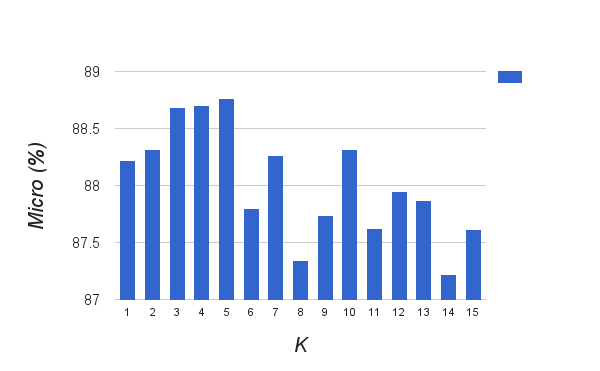
\includegraphics[width=\linewidth]{./k_effect.png}
\caption{Effect of parameter $K$ on entity linking accuracy.
Trained on CoNLL train and tested on CoNLL test-a.}
\label{fig:k_effect}
\end{figure}
}
% PGF plot version of the figure
{
\pgfplotsset{every tick label/.append style={font=\tiny}}
\begin{figure}[t!]
\centering
\resizebox {\columnwidth} {!} {
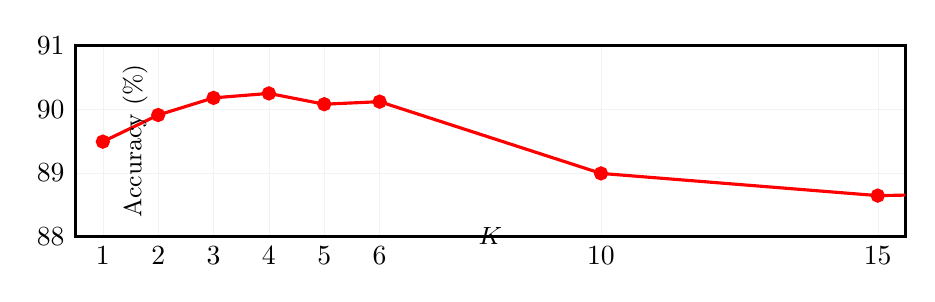
\begin{tikzpicture}
  \begin{axis}[
   %title  = Effect of K,
   width = \columnwidth,
   height=4cm,
%    ybar,
 %   bar width = 0.2cm,
    %x axis line style = { opacity = 0 },
    %axis y line       = none,
    tickwidth         = 0pt,
    xmin=0.5,xmax=15.5,
    ymin=88,ymax=91,
    grid=both,
    grid style={line width=.1pt, draw=gray!10},
    x label style={at={(axis description cs:0.5,0.1)},anchor=north},
    y label style={at={(axis description cs:0.1,.5)},anchor=south},
    xlabel={\small $K$},
    ylabel={\small Accuracy (\%)},
    mark size=2.0pt,
    line width=1.0pt,
   % enlarge y limits  = 0.2,
    xtick = data,
  ]
  \addplot [line width=0.4mm, red, mark=*, mark options=solid] coordinates { 
    (1,89.49) (2,89.91)  (3,90.18) (4,90.25) (5,90.08) (6,90.12) (10,88.99) (15,88.64) (20,88.72)
  };
  \pgfresetboundingbox
  %\addplot coordinates { (20,1)         (15,2)
   %                      (60,3)   (75,4)  };
 % \legend{Topics, Posts}
  \end{axis}
\end{tikzpicture}
}
\caption{Effect of parameter $K$ on entity linking accuracy.
Trained on CoNLL train and tested on CoNLL test-a. \label{fig:k_effect}}
\end{figure}
}

%(1,89.72) (2, 89.77) (3, 90.39) (4, 90.39) (5, 90.52)   (6,90) (7,90) (8,90) (9,90) (10,90)   (11,90) (12,90) (13,90) (14,90) (15,90)};


In \secref{sec:soft_attention} we proposed an extension of softmax smoothing to the $K$ attention case. In our experiments 
we cross-validated over a wide range of $\beta$ values, including $\beta=\infty$ which corresponds to taking
the exact sum of $K$ largest values. We found that the optimal value in most cases was large: $\beta=10, 100$, or even $\infty$. This suggests that a {\em hard} attention model, where exactly $K$ mentions are picked is adequate in the current settings.

%\subsection{Examples of gains (and losses)}



%%% Local Variables: ***
%%% mode:latex ***
%%% TeX-master: "main.tex"  ***
%%% tex-main-file: "main.tex"  ***
%%% End: ***

\section{Conclusion}
\label{sec:End}

We have described an attention-based approach to collective entity resolution,
motivated by the observation that a non-salient entity in a long document may
 only have relations to a small subset of other entities. 
 We explored two approaches to attention: a multi-focus attention model
 with tractable inference decomposed over mentions, and a single-focus
model with global inference implemented using belief propagation.
%Two implementation
%of the approach were described: one which uses inference on star shaped graphs, and one
% which does global inference using belief propagation.
Our empirical results show that the methods results in significant performance gains
across several benchmarks. 

Experiments in varying the size of the attention beam $K$ in the star-shaped model suggest that
 multi-focus attention is beneficial.
 % and performs well when coupled with
 % simple tractable inference, decomposed over mentions. 
 It is of course possible to extend the global
 single-link model to the multi-focus case, by modifying the model
 factors and resulting messages. 
 However, the simplicity of the star-shaped model, its empirical effectiveness, and ease of learning parameters make it an attractive approach for easily incorporating attention into existing resolution models. The model can also readily be applied 
to other structured prediction problems in language processing, such as
selecting antecedents in coreference resolution.


Deep learning has recently been used in mutliple NLP applications, including parsing \cite{chen2014fast} and translation \cite{bahdanau2014neural}. 
Learning the local and pairwise scores in our model using a deep architecture rather
than a linear model would likely lead to performance improvements.
The star-shaped model is particularly amenable to this architecture, as it can be implemented via
a feed-forward sequence of operations (including sorting, which can be implemented with soft-max gates).

Finally, one may consider a more elaborate model in which attention
 depends on the current state of the system; 
 for example, the state can summarize the mention context.
%For example, this can allow the attention to change according to context. 
The dynamics of the underlying state can be modeled by
recurrent neural networks or LSTMs \cite{bahdanau2014neural}. 

In conclusion, we have shown that attention is an effective mechanism for improving entity resolution models, and that it can be implemented
via a simple inference mechanism, where model parameters can be easily learned. 
 


\comment{
 two new approaches to modeling coherence for entity
resolution.  While most existing systems consider all relations
between entity candidates for a document to assign a coherence score
to a candidate, we use a novel attention mechanism to select the most
relevant relations.  Our experimental results support \hl{do they?}
the premise that the inclusion of all relations can hurt performance.
Our models improve the performance of a baseline system on three
evaluation benchmarks, and our best multi-focal attention model
achieves state-of-the-art results on standard benchmarks against
highly competitive recently built systems.
}
\section{Proof of Proposition \ref{prop:softkmax}}
Assume w.l.o.g. that $z_i$ are sorted in decreasing order. 
Begin with the optimization problem in \eqref{eq:softkmax_opt}. Introduce the following Lagrange multipliers: $\lambda$ 
for the $\sum_i\mu_i=K$ constraint, and $\alpha_i\geq 0 $ for the $\mu_i \leq 1$ constraint. We can ignore the $\mu_i \geq 0 $
constraint, as it will turn out to be satisfied. Denote the corresponding Lagrangian by $L(\mu,\lambda,\alpha)$. We will show the result
by using the convex dual  $g(\lambda,\alpha) = \min_{\mu} L(\mu,\lambda,\alpha)$ and the fact that the solution of  \eqref{eq:softkmax_opt}
is $\max_{\lambda,\alpha} g(\lambda,\alpha)$.

Minimizing $L$ with respect to $\mu_i$ yields:
\be
\mu_i = e^{\beta z_i -1 + \beta \lambda - \beta \alpha_i}
\label{eq:opt_mu}
\ee
From this we can obtain the convex dual:
\be
g(\lambda,\alpha) = -\lambda K  + \beta^{-1} \sum_i   e^{\beta z_i -1 + \beta \lambda - \beta \alpha_i}  + \sum_i \alpha_i 
\ee
Maximizing this with respect to $\lambda$ yields the maximizing $\lambda^*$:
\be
\lambda^* = \beta^{-1}  \log{\frac{K}{ \sum_i e^{\beta z_i -1-\beta \alpha_i}} }
\ee
We can now express $g$ as a function of only $\alpha$
\be
g(\alpha) =  K\beta^{-1}   \log{\frac{ \sum_i e^{\beta z_i-\beta \alpha_i}}{K}} + \sum_i \alpha_i
\ee
Next, we maximize the above with respect to $\alpha\geq 0 $. Introduce Lagrange multipliers 
$\gamma_i$ for the constraint $\alpha_i \geq 0$ and the corresponding Lagrangian $\bar{L}(\alpha,\gamma)$. We next propose
a solution for $\alpha,\gamma$ and show that it satisfies the KKT conditions. Minimizing $\bar{L}$ wrt $\alpha$ we can characterize
the optimal $\gamma$ as:
\be
\gamma_i = -K \frac{e^{\beta z_i -\beta \alpha_i}}{\sum_i e^{\beta z_i-\beta \alpha_i}} + 1 
\label{eq:opt_gamma}
\ee
Define: 
\be
c ={1\over \beta} \log{\sum_{i=K}^n e^{\beta z_i}}
\ee
Set $\alpha_i$ as follows:
\be
\alpha_i = 
\left\{
\begin{array}{ll}
z_i - c & i=1,\ldots, K -1  \\
0 & i = K,\ldots, n
\end{array}
\right.
\label{eq:opt_alpha}
\ee
It can now be confirmed that the $\alpha,\gamma$ from Equations \ref{eq:opt_alpha} and \ref{eq:opt_gamma} satisfy the KKT conditions. Plugging the $\alpha $ value into $g(\alpha)$ yields the solution in the proposition. The result from the gradient follows from the fact that $L(\mu,\lambda,\alpha)$ is uniquely  minimized by \eqref{eq:opt_mu} and this is the subgradient (and due to uniqueness also the gradient) of $\samax(z)$ with respect to $z$.

%\section*{Acknowledgments}
%Do not number the acknowledgment section.

%\begin{small}
\bibliography{refs}
\bibliographystyle{acl2016}
%\end{small}

\end{document}
